
Throughout this paper, we use \emph{conventional digital computers} as an umbrella term for stored-program machines (e.g., von Neumann-style architectures): at the theory level they are commonly abstracted as random-access machines with an instruction set architecture, and at the systems level they are typically realized through layered operating-system/application stacks. Such systems separate computation, memory, and I/O.
Our motivating question is whether a single set of weights can internalize these roles inside one latent runtime state, rather than relying on an external execution environment (e.g., OS/simulator) to carry executable state.
We model a video-based neural computer (NC) prototype as a learned latent-state system that folds these roles into an update-and-render loop.

\begin{figure}[h!]
  \centering
  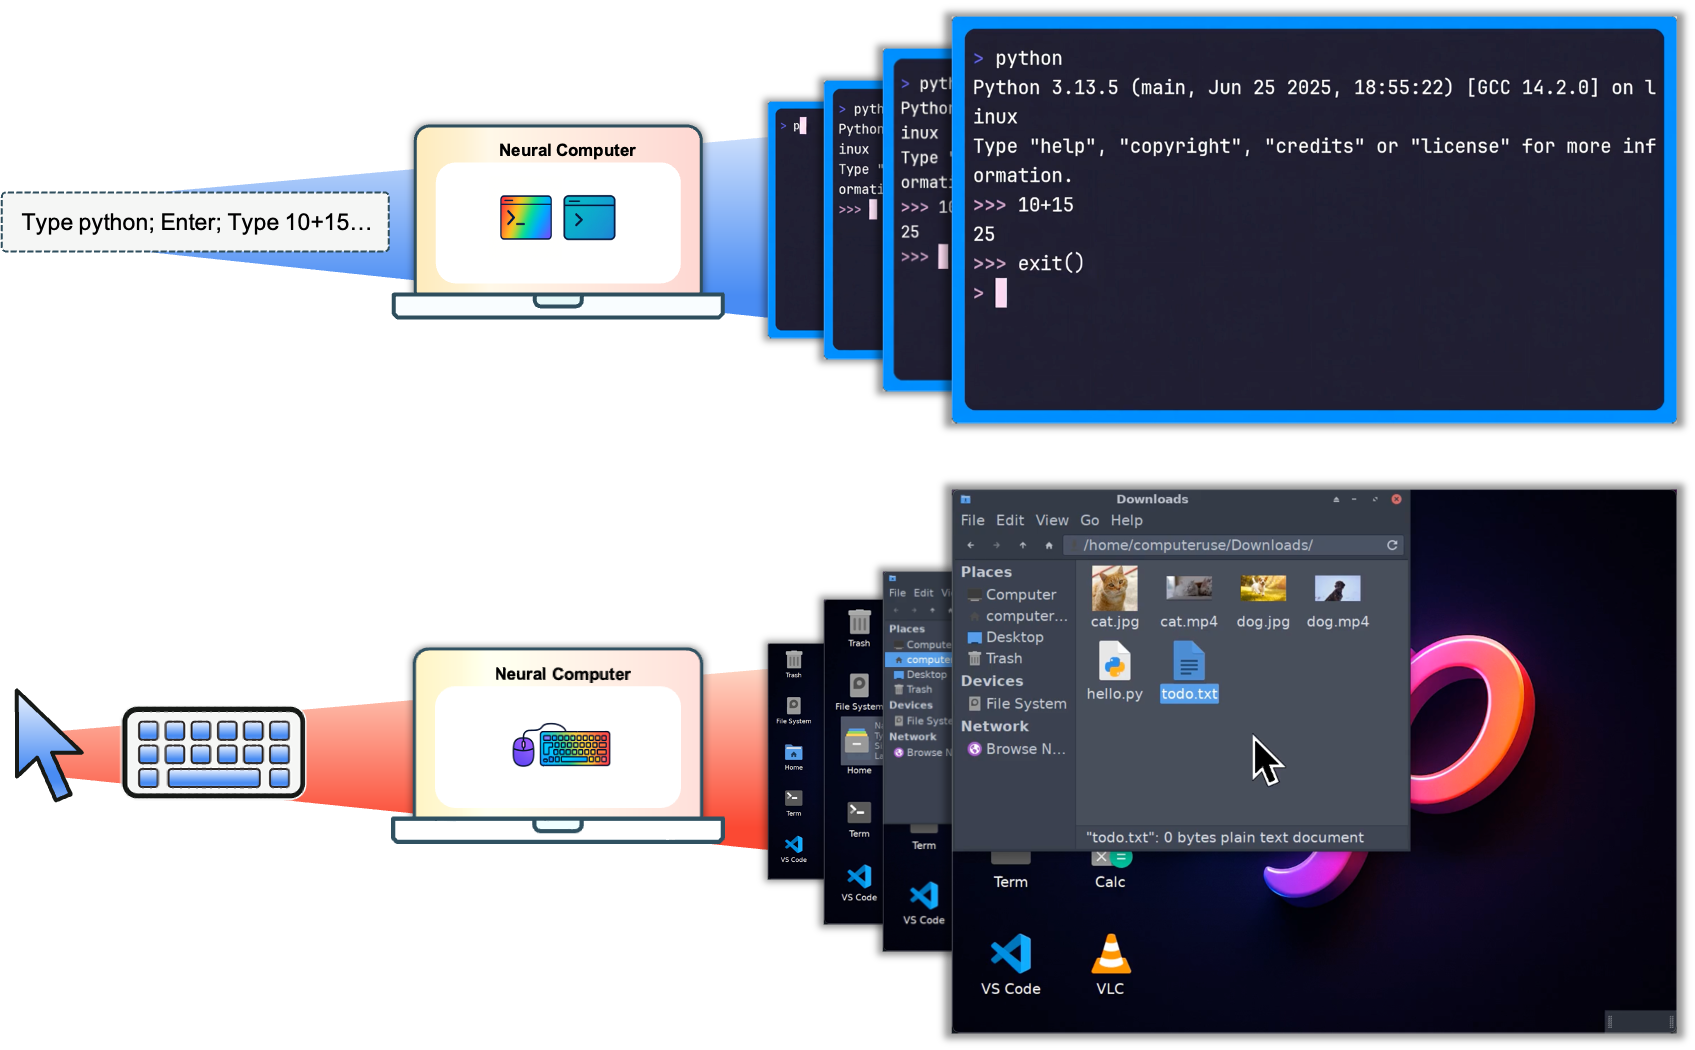
\includegraphics[width=1.0\linewidth]{assets/nc_general.png}
\caption{\textbf{Neural computers across interfaces.}
Given a prompt or action stream, an NC rolls out future interface frames for \cligenGeneralLogo{}/\cligenCleanLogo{}\,\nccligen{} (top) and \guiworldLogo{}\,\ncguiworld{} (bottom).
Logos denote datasets; \nccligen{} and \ncguiworld{} are the corresponding models trained on those datasets.
It models terminal or desktop dynamics.}
  \label{fig:nc-general}
\end{figure}

Specifically, an NC updates a latent runtime state from the current observation and conditioning input, and then predicts (or samples) the next observation.
In this paper, we treat screen frames as observables and define actions as time-indexed conditions. More broadly, the NC framework can accommodate various other modalities and structural representations for both observables and actions.
Given an initial screen frame $x_0$ and conditioned on user action $u_t$ at iteration $t$, an NC updates its memory state and samples the next frame $x_{t+1}$.
% Formally, an NC defined by an initial memory state $h_0$, an update function $F_\theta$, and a decoder $G_\theta$ operates as follows:
Formally, an NC defined by an initial memory state $h_0$, an update function $F_\theta$, and a decoder $G_\theta$ operates as follows, where $G_\theta$ parameterizes a distribution over next frames:


\begin{align}
h_t &= F_\theta(h_{t-1}, x_t, u_t), \qquad x_{t+1} \sim G_\theta(h_t).
\label{eq:wm}
\end{align}

\noindent\textit{Notation.} We use $h_t$ for the NC latent runtime state and reserve $z$ for VAE/video latents used in diffusion-style video models (e.g., \Cref{section:impl-guiworld}). 

We cast this update-and-render loop as a world model of a computer interface, where $x_t$ are observations and $u_t$ provides conditioning.
In world-modeling terminology, the input sequence $\{u_t\}$ is referred to as a conditioning stream.
Under this view, an NC is not merely a predictor but a learned runtime mechanism: the latent state $h_t$ carries executable context; $F_\theta$ integrates new observations and inputs, and $G_\theta$ renders the next frame.
Auxiliary heads can encode and decode prompts, buffers, or action traces, shifting functionality that would traditionally live in OS queues, device drivers, and UI toolkits into latent-state dynamics.

\subsection{Related Work}
\label{section:prelim-related}

Early neuromorphic designs~\citep{mead2012analog} explored neural computation as a physical substrate.
Differentiable memory and program-execution architectures, including Neural Turing Machines~\citep{graves2014neural},
Differentiable Neural Computers~\citep{graves2016hybrid}, and Neural Programmer-Interpreters~\citep{reed2015neural}, showed that neural controllers with memory can execute structured procedures.
Differentiable world models~\citep{schmidhuber1990making,schmidhuber2015learning} learn neural representations of environment dynamics, and inspire our update-and-render formulation.
%
Latent video and world models~\citep{ha2018world,hafner2019learning,hafner2019dream,bruce2024genie} extend these ideas to embodied control and interactive environments.
Genie~3~\citep{bruce2024genie}, in particular, frames such models as agent-training substrates with improved physical consistency.
More recently, high-capacity generators such as Veo~3~\citep{google_veo3_1_2025} and Sora~2~\citep{openai_sora2_2025} emphasize open-ended, photorealistic simulation.
In parallel, systems such as NeuralOS~\citep{rivard2025neuralos} and Imagine with Claude~\citep{anthropic_claude_sonnet4_5_2025} bring model-based conditioning to desktop and DOM-style interfaces.
%
Building on this trajectory, we study two NC instantiations for CLI and GUI with interface-specific conditioning, supported by a shared data engine and a staged roadmap toward the CNC vision.
